\documentclass[11pt]{article}
\usepackage[margin=1in]{geometry}
\usepackage{times}
\usepackage{amsmath,amssymb}
\usepackage{graphicx}
\usepackage{booktabs}
\usepackage{hyperref}
\usepackage[numbers,sort&compress]{natbib}
\usepackage{microtype}
\usepackage{caption}
\usepackage{subcaption}
\usepackage{xcolor}

\graphicspath{{figures/}}

\hypersetup{
  colorlinks=true,
  linkcolor=blue!60!black,
  citecolor=blue!60!black,
  urlcolor=blue!60!black,
}

\title{\textbf{Learning Combinatorial Distance Heuristics:}\\[4pt]
Optimizer and Hyperparameter Effects on a\\
2$\times$2$\times$2 Rubik's Cube Solver}
\author{Cole McGuire\\[2pt]
\small Colorado School of Mines\\
\small Special Topics: Numerical Optimization}
\date{Spring 2026}

% ============================================================
\begin{document}
\maketitle

% ---- Abstract -----------------------------------------------
\begin{abstract}
We study the numerical optimization of a small transformer trained to approximate
BFS optimal distance on the 2$\times$2$\times$2 Rubik's cube---a combinatorial
domain where ground-truth solutions are exactly computable.
We compare three first-order optimizers (AdamW, Adam, SGD with momentum) and
three learning rate schedules (cosine annealing, constant, step decay), conduct
a hyperparameter sensitivity analysis over model width and weight decay, analyze
the quality of the learned distance heuristic relative to BFS ground truth, and
visualize the loss landscape via filter-normalized random directions
\cite{li2018landscape}.
Our results show that \textbf{[fill in after experiments]}.
The cube's controlled structure enables unusually clean analysis of
optimizer behavior in the non-convex setting.
\end{abstract}

% ============================================================
\section{Introduction}
\label{sec:intro}

Training a deep neural network is fundamentally a non-convex numerical
optimization problem. The choice of optimizer and learning rate schedule
determines not only whether the model converges, but how quickly, to what
quality of solution, and with what sensitivity to hyperparameters.
Understanding these dynamics is difficult in general: loss surfaces are
intractable, ground-truth optimal performance is unknown, and empirical
comparisons on large benchmarks conflate optimizer effects with task difficulty.

The 2$\times$2$\times$2 Rubik's cube offers a rare controlled setting.
Its full state space---roughly 3.7 million reachable positions---is small
enough that the true minimum number of moves to solve any state (the
\emph{optimal distance}) can be computed exactly via bidirectional BFS.
God's number for the 2$\times$2$\times$2 is 11 moves in the half-turn metric
\cite{agostinelli2019deepcubea}.
A neural network trained to predict this distance is therefore learning to
approximate a \emph{known} function with structured geometry:
distance is 0 at the solved state, increases monotonically under scrambling,
and is symmetric under rotational equivalences of the cube.

This paper frames transformer training on optimal-distance classification as a
numerical optimization problem and asks three questions:
(1) How do the optimizer algorithm and learning rate schedule affect convergence
speed and final accuracy?
(2) How sensitive is training to hyperparameter choices (model width, weight
decay)?
(3) What is the quality of the learned heuristic relative to exact BFS, and what
does the loss landscape look like in the neighborhood of the solution?

The latter question connects to combinatorial search: a learned distance
heuristic that consistently underestimates true distance would be
\emph{admissible} in the sense of A* \cite{hart1968astar}, enabling provably
optimal search with reduced node expansions. We measure empirically whether
our trained model achieves this property.

% ============================================================
\section{Related Work}
\label{sec:related}

\paragraph{Adaptive gradient methods.}
Stochastic gradient descent with momentum \cite{polyak1964momentum,rumelhart1986backprop}
remains a strong baseline but requires careful learning rate tuning.
Adam \cite{kingma2015adam} introduced per-parameter adaptive learning rates via
first and second moment estimates, substantially reducing sensitivity to the
global learning rate.
AdamW \cite{loshchilov2019adamw} decoupled weight decay from the gradient
update, correcting a subtle regularization failure in Adam where L2 penalty
interacts with the adaptive step sizes.
On most deep learning benchmarks AdamW is the current default; whether this
advantage holds on small, structured combinatorial tasks is an open question.

\paragraph{Learning rate scheduling.}
Cosine annealing \cite{loshchilov2017sgdr} decays the learning rate from an
initial value to a minimum following a half-cosine curve, smoothly reducing
the step size as the optimizer approaches a local minimum.
Step decay applies a fixed multiplicative reduction at preset epoch milestones,
and constant schedules serve as a baseline.
Schedule choice interacts strongly with optimizer: adaptive methods are less
sensitive to the global LR trajectory, while SGD-like methods depend heavily
on scheduling to avoid divergence or slow final convergence.

\paragraph{Loss landscape geometry.}
Li et al.\ \cite{li2018landscape} introduced filter normalization to visualize
loss surfaces in directions that are scale-invariant with respect to the network
weights. Their method plots loss along two random directions in parameter space,
scaled so that each perturbation direction has the same Frobenius norm as the
corresponding filter. This reveals whether solutions sit in wide, flat basins
(empirically associated with better generalization) or sharp narrow minima.
Goodfellow et al.\ \cite{goodfellow2015landscape} established that the loss
along the linear path between two random initializations and a trained solution
is often monotone, suggesting the optimization trajectory is simpler than the
full non-convex landscape implies.

\paragraph{Learned heuristics for combinatorial search.}
DeepCubeA \cite{agostinelli2019deepcubea} trained a deep residual network to
predict distance-to-goal on the 3$\times$3$\times$3 cube via self-supervised
reverse BFS, then used the predictions as a heuristic in BWAS (Batch-Weighted
A*) to find optimal solutions. Their model is not admissible by construction
but achieves optimal solutions in practice by combining the heuristic with
tree search. Our setting is simpler---we train by direct supervision on BFS
distances---but the heuristic quality analysis (admissibility, MAE by distance)
connects directly to this body of work.

\paragraph{Training dynamics and grokking.}
Power et al.\ \cite{power2022grokking} showed that small transformers trained
on modular arithmetic can exhibit sudden generalization long after training
loss has converged---a phenomenon called grokking. Nanda et al.\
\cite{nanda2023grokking} identified the underlying algorithmic mechanism via
mechanistic interpretability. We examine whether similar dynamics appear in
our combinatorial setting.

% ============================================================
\section{Methodology}
\label{sec:method}

\subsection{Problem Formulation}

Let $\mathcal{S}$ denote the set of 2$\times$2$\times$2 Rubik's cube states
(approximately 3.7 million reachable positions). For each state
$s \in \mathcal{S}$, let $d^*(s) \in \{0, 1, \ldots, 11\}$ be the BFS optimal
distance to the solved state. We represent each state as a 144-dimensional
one-hot vector: 24 sticker positions, each encoded as a 6-class one-hot over
colors. The learning problem is 12-class classification:
\begin{equation}
  \hat{d}(s; \theta) = \arg\max_{k} f_k(s;\, \theta),
\end{equation}
where $f(s;\theta) \in \mathbb{R}^{12}$ is the network output and $\theta$
denotes all learnable parameters. We minimize the weighted cross-entropy loss
\begin{equation}
  \mathcal{L}(\theta) = -\frac{1}{N}\sum_{i=1}^{N}
    w_{d^*(s_i)} \log \frac{e^{f_{d^*(s_i)}(s_i;\theta)}}
                            {\sum_{k=0}^{11} e^{f_k(s_i;\theta)}},
\end{equation}
where $w_k \propto 1/\text{count}(k)$ are inverse-frequency class weights to
compensate for the uneven distribution of BFS distances in uniformly scrambled
states (distances near God's number are rarer).

\subsection{Model Architecture}

We use a small transformer with a single input token. The 144-dim state vector
is linearly projected to a $d_\text{model}$-dimensional embedding, passed
through $L$ transformer blocks (each with multi-head self-attention and an MLP
sublayer), and then decoded by a linear head to 12 logits. Since there is only
one input token, the attention sublayers are degenerate (weights always 1.0);
the model computes almost entirely through the MLP sublayers. The default
configuration is $d_\text{model} = 128$, $L = 4$ layers, $H = 4$ heads,
yielding approximately 200k parameters.

\subsection{Optimizers}

We compare three first-order optimization algorithms.

\paragraph{SGD with momentum.}
\begin{equation}
  v_{t+1} = \mu v_t + \nabla_\theta \mathcal{L}(\theta_t), \qquad
  \theta_{t+1} = \theta_t - \eta\, v_{t+1},
\end{equation}
where $\eta$ is the learning rate and $\mu = 0.9$ is the momentum coefficient
\cite{polyak1964momentum}. Weight decay is applied as an L2 penalty on the loss.

\paragraph{Adam.}
\begin{align}
  m_{t+1} &= \beta_1 m_t + (1 - \beta_1)\, g_t, \\
  v_{t+1} &= \beta_2 v_t + (1 - \beta_2)\, g_t^2, \\
  \theta_{t+1} &= \theta_t - \eta \frac{\hat{m}_{t+1}}{\sqrt{\hat{v}_{t+1}} + \epsilon},
\end{align}
where $g_t = \nabla_\theta \mathcal{L}(\theta_t)$, $\hat{m}$ and $\hat{v}$ are
bias-corrected estimates, and default hyperparameters are
$\beta_1 = 0.9$, $\beta_2 = 0.999$, $\epsilon = 10^{-8}$ \cite{kingma2015adam}.
Adam with weight decay adds $\lambda\theta$ to the gradient before the update,
coupling the decay with the adaptive step size.

\paragraph{AdamW.}
AdamW \cite{loshchilov2019adamw} decouples weight decay from the gradient
update:
\begin{equation}
  \theta_{t+1} = (1 - \eta\lambda)\,\theta_t
                 - \eta \frac{\hat{m}_{t+1}}{\sqrt{\hat{v}_{t+1}} + \epsilon}.
\end{equation}
This is the only modification from Adam; the effect is that weight decay acts
as a multiplicative shrinkage independent of the per-parameter adaptive step
size, restoring its intended regularization behavior.

\subsection{Learning Rate Schedules}

\paragraph{Cosine annealing.}
The learning rate follows a half-cosine decay from $\eta_0$ to $\eta_\text{min}$:
\begin{equation}
  \eta_t = \eta_\text{min} + \tfrac{1}{2}(\eta_0 - \eta_\text{min})
           \left(1 + \cos\!\left(\frac{\pi t}{T}\right)\right),
\end{equation}
where $T$ is the total number of epochs and we set $\eta_\text{min} = \eta_0 / 20$
\cite{loshchilov2017sgdr}.

\paragraph{Step decay.}
The learning rate is multiplied by a factor $\gamma = 0.3$ every 10 epochs,
giving $\eta_t = \eta_0 \cdot \gamma^{\lfloor t/10 \rfloor}$.

\paragraph{Constant.}
$\eta_t = \eta_0$ throughout training, providing a baseline that isolates
optimizer behavior from schedule effects.

\subsection{Heuristic Quality Metrics}

Beyond classification accuracy, we evaluate the learned distance function as a
heuristic $h(s) = \hat{d}(s)$ for combinatorial search using three metrics:

\begin{enumerate}
  \item \textbf{Mean absolute error (MAE)} by true distance:
    $\text{MAE}(k) = \mathbb{E}[|\hat{d}(s) - k| \mid d^*(s) = k]$.
  \item \textbf{Admissibility}: a heuristic is admissible if it never
    overestimates, i.e., $\hat{d}(s) \leq d^*(s)$ for all $s$.
    We measure the fraction of states where the model overestimates.
  \item \textbf{Per-distance accuracy}: how often the model's predicted class
    exactly matches the BFS distance.
\end{enumerate}

\subsection{Loss Landscape Visualization}

Following Li et al.\ \cite{li2018landscape}, we visualize the loss surface
around the trained weights $\theta^*$ by evaluating the loss on a 2D grid:
\begin{equation}
  \mathcal{L}(\alpha, \beta) = \mathcal{L}(\theta^* + \alpha\,\delta + \beta\,\eta),
\end{equation}
where $\delta, \eta$ are random directions in parameter space normalized
via filter normalization: each filter in $\delta$ (resp.\ $\eta$) is scaled
to have the same Frobenius norm as the corresponding filter in $\theta^*$,
making the visualization scale-invariant with respect to network width.

% ============================================================
\section{Experiments}
\label{sec:experiments}

\subsection{Experimental Setup}

All experiments use the same 2$\times$2$\times$2 cube dataset: 300k training
samples, 30k validation samples, drawn from scrambles of depth 1--11 via BFS.
The default model configuration is $d_\text{model} = 128$, 4 layers, 4 heads.
Unless varied, the default optimizer is AdamW with $\eta_0 = 10^{-3}$,
$\lambda = 10^{-4}$, and cosine annealing over 30 epochs with batch size 512.
Each experiment is run once; results are saved to JSON and figures are generated
reproducibly from cached results. All training was performed on
\texttt{[device]} in approximately \texttt{[X]} minutes per run.

\subsection{Optimizer Comparison}

We train three models under AdamW, Adam, and SGD with momentum, holding the
schedule (cosine annealing) and all other hyperparameters fixed. For SGD we
use $\eta_0 = 0.05$, selected by a short grid search over
$\{0.01, 0.05, 0.1\}$; AdamW and Adam use $\eta_0 = 10^{-3}$.

% ---- Figure placeholder ----
\begin{figure}[h]
  \centering
  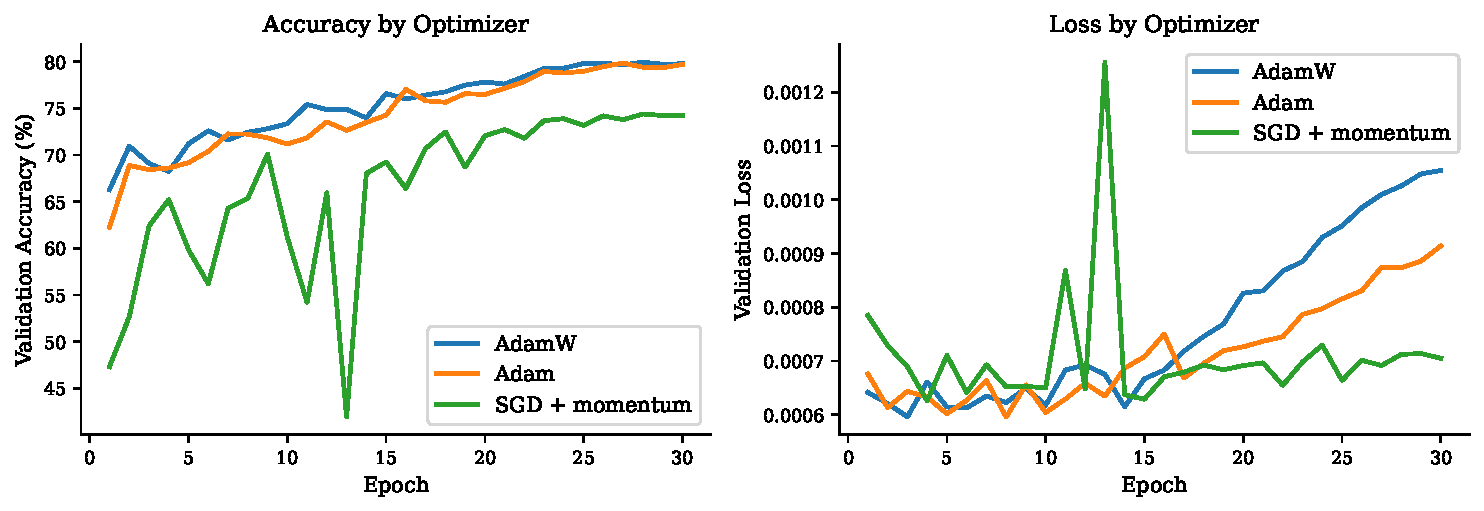
\includegraphics[width=\linewidth]{optimizer_comparison}
  \caption{Validation accuracy (left) and validation loss (right) over 30
    training epochs for AdamW, Adam, and SGD with momentum under cosine
    annealing. \textbf{[Add interpretation after running experiments.]}}
  \label{fig:optimizer}
\end{figure}

\textbf{[Analysis to be written after running experiments.]}

\subsection{Learning Rate Schedule Ablation}

Holding optimizer fixed to AdamW, we compare cosine annealing, step decay
($\gamma = 0.3$ every 10 epochs), and a constant schedule.

\begin{figure}[h]
  \centering
  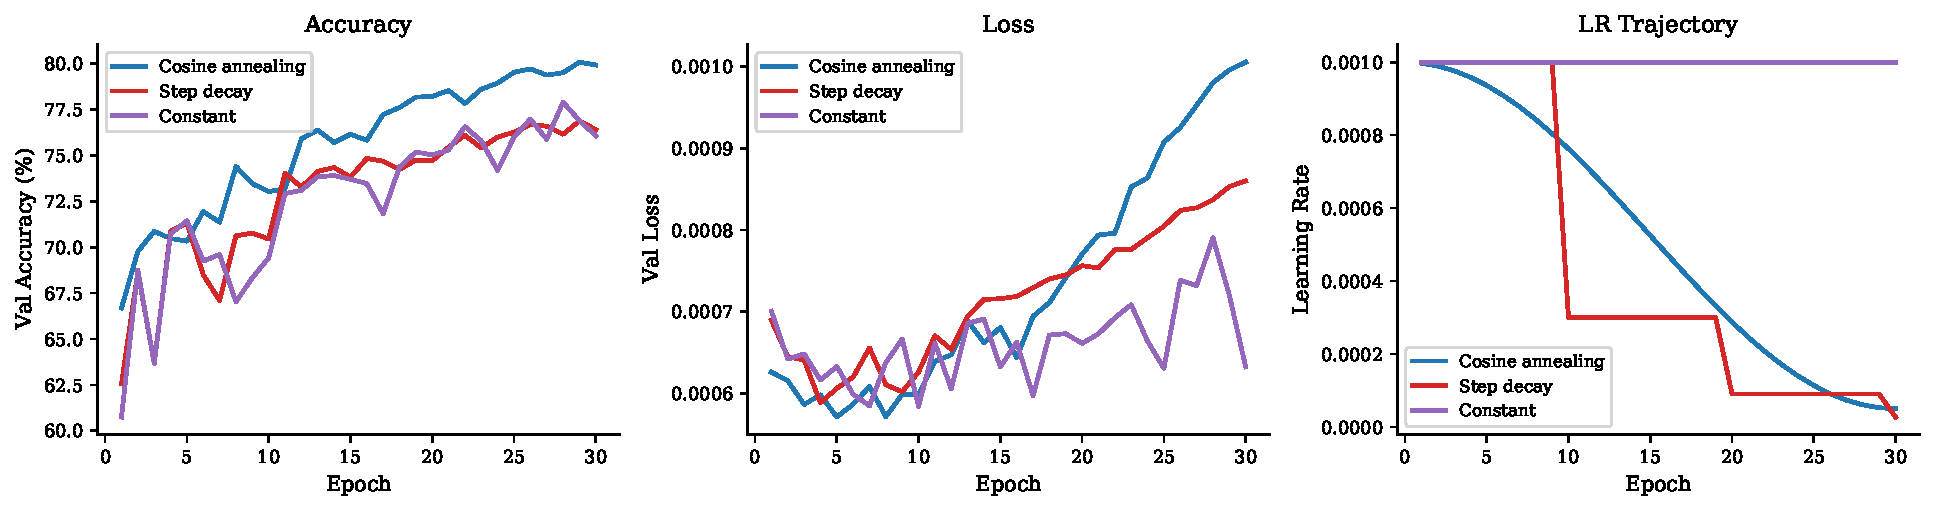
\includegraphics[width=\linewidth]{schedule_comparison}
  \caption{Validation accuracy over training for three learning rate schedules
    under AdamW. Right panel shows the LR trajectory for each schedule.
    \textbf{[Add interpretation.]}}
  \label{fig:schedule}
\end{figure}

\textbf{[Analysis to be written after running experiments.]}

\subsection{Hyperparameter Sensitivity}

We sweep two hyperparameters: model width ($d_\text{model} \in \{64, 128, 256\}$,
fixing $L = 4$, $H = 4$) and weight decay
($\lambda \in \{0, 10^{-4}, 10^{-3}, 10^{-2}\}$, fixing $d_\text{model} = 128$).

\begin{figure}[h]
  \centering
  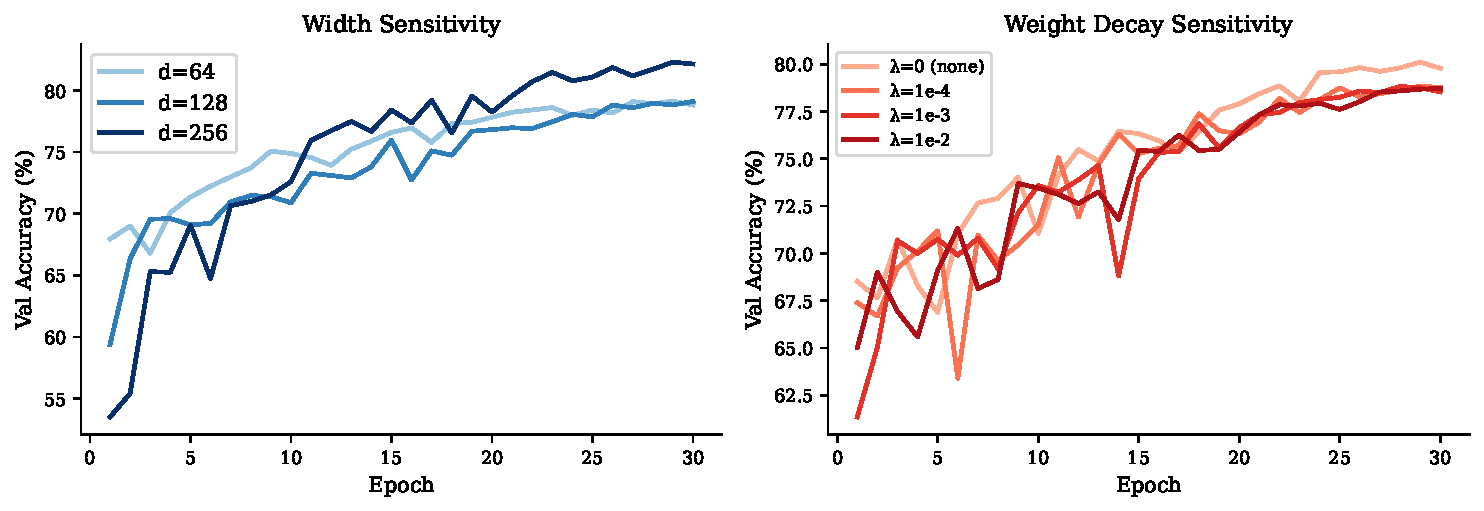
\includegraphics[width=\linewidth]{hyperparameter_sensitivity}
  \caption{Final validation accuracy as a function of model width (left) and
    weight decay (right). \textbf{[Add interpretation.]}}
  \label{fig:hyperparam}
\end{figure}

\textbf{[Analysis to be written after running experiments.]}

\subsection{Learned Heuristic Quality}

Using the best-trained model (AdamW, cosine annealing, $d_\text{model} = 128$),
we evaluate heuristic quality on the full 30k validation set.

\begin{figure}[h]
  \centering
  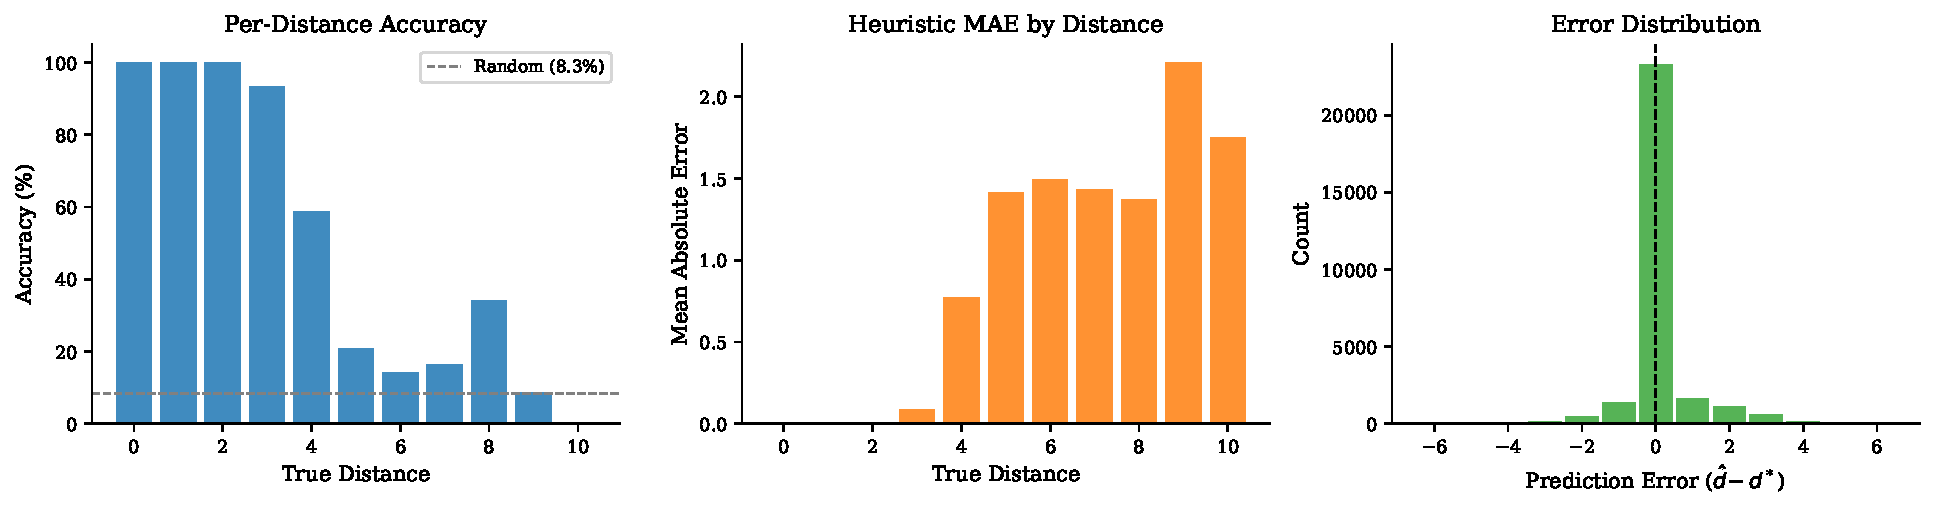
\includegraphics[width=\linewidth]{heuristic_quality}
  \caption{Left: per-distance classification accuracy. Center: mean absolute
    error of predicted distance by true distance. Right: distribution of
    prediction errors ($\hat{d} - d^*$); negative values indicate
    underestimates (admissible), positive values indicate overestimates
    (inadmissible). \textbf{[Add interpretation.]}}
  \label{fig:heuristic}
\end{figure}

\textbf{[Analysis to be written after running experiments.]}

\subsection{Loss Landscape}

\begin{figure}[h]
  \centering
  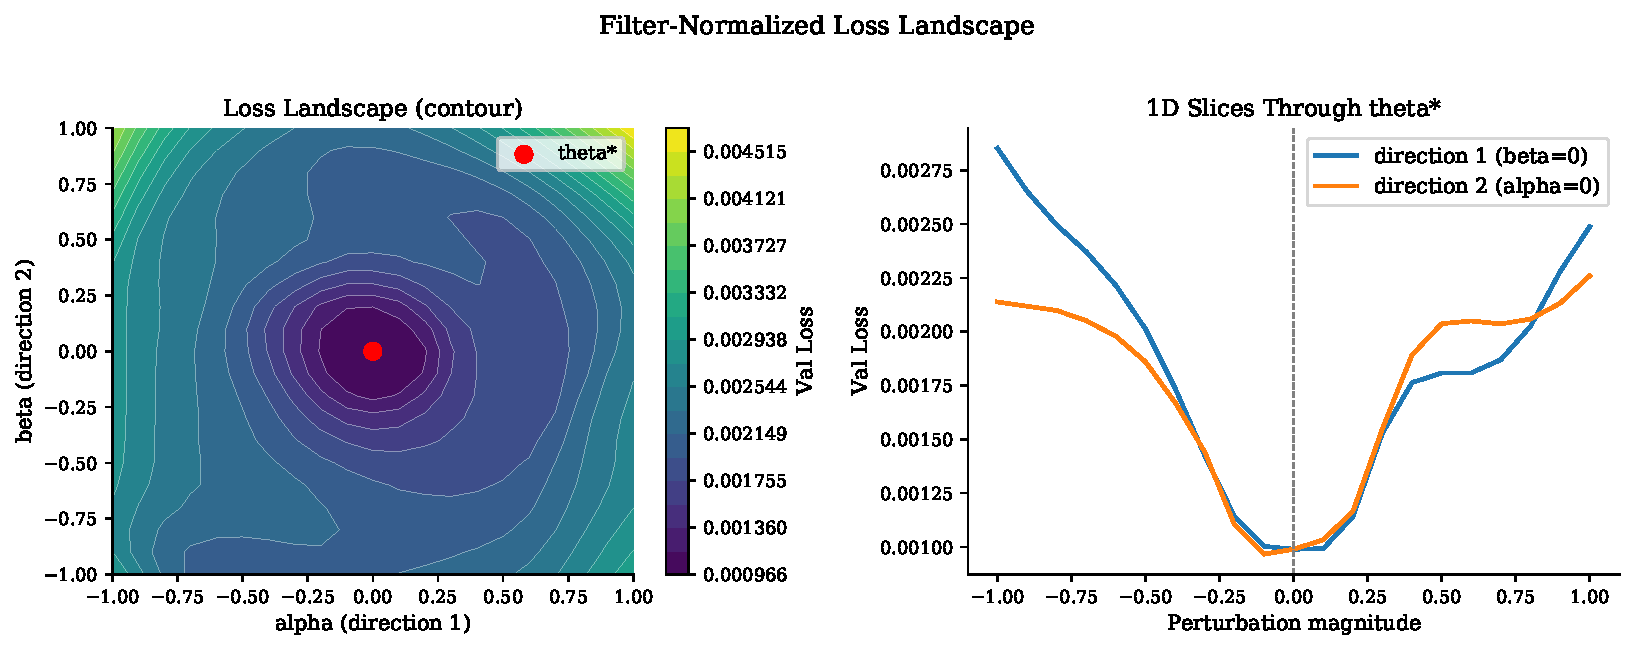
\includegraphics[width=0.7\linewidth]{loss_landscape}
  \caption{Filter-normalized loss landscape around the AdamW solution
    $\theta^*$. The surface is evaluated on the validation set over a
    $21 \times 21$ grid of perturbation magnitudes $\alpha, \beta \in [-1, 1]$.
    \textbf{[Add interpretation.]}}
  \label{fig:landscape}
\end{figure}

\textbf{[Analysis to be written after running experiments.]}

% ============================================================
\section{Conclusion}
\label{sec:conclusion}

\textbf{[To be written after experiments are complete.]}

Key points to address:
\begin{itemize}
  \item Which optimizer converged fastest / to the best solution, and why the
    result is or is not surprising for this task structure.
  \item Effect of schedule; whether cosine annealing's advantage over constant
    LR is large or small.
  \item Hyperparameter sensitivity: is this task ``easy to optimize'' in the
    sense that a wide range of hyperparameters reaches similar performance?
  \item Heuristic quality: is the model admissible? Where does it fail most?
  \item What the loss landscape reveals about the geometry of the solution.
  \item Limitations: single run per configuration (no error bars), 2$\times$2$\times$2
    only (smaller than practical puzzles), single architecture (MLP-dominated transformer).
  \item Future work: A* search using the learned heuristic, scaling to
    3$\times$3$\times$3, warm restarts (SGDR).
\end{itemize}

% ============================================================
\bibliographystyle{plainnat}
\bibliography{references}

\end{document}
